\thispagestyle{empty}
\null
\vfill
\begin{center}

   
\includegraphics[width=1.0\textwidth]{res/nordigavisor.jpg}
   \section{Nördiga visor}

\end{center}
\vfill
\newpage

\subsection{IQ-test}
\vfill
\begin{center}

   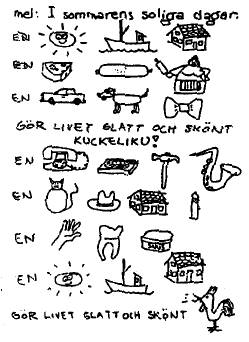
\includegraphics[width=1.0\textwidth]{res/iqtest.png}

\end{center}
\vfill
\newpage

\subsection{CVS-visan}
\textit{Mel: Odefinierad/Valfri}\\
\index[alfa]{CVS-visan}
\index[anfa]{Status told there's something new...}
\begin{parse lines}[\noindent]{#1\\}

Status told there's something new
UPDATE, UPDATE, UPDATE, COMMIT

Many files or just a few
UPDATE, UPDATE, UPDATE, COMMIT

We don't need to hope and pray
UPDATE, UPDATE, UPDATE, COMMIT

'cause we work the clever way
UPDATE, UPDATE, UPDATE, COMMIT
\end{parse lines}

\noindent\textit{(Rad i gemener sjunges av försångare)\\
Sjungs av Lars Bendix på någon föreläsning i kursen EDA260.}




\subsection{D-visor}
\textit{Mel: Row, row, row your boat}\\
\index[alfa]{D-visor}
\index[anfa]{$\rho\  \rho\  o...$}


\noindent $\rho\  \rho\  o \\
\lambda\  \sigma\  \xi \\
\nu\  \varepsilon\  \delta\  \mu\  \varphi \\
\theta\  \kappa\  \pi $\\


\subsection{En komplex värld}
\textit{Mel: En helt ny värld}\\
\index[alfa]{En komplex värld}
\index[anfa]{Alla jävla bevis...}
\begin{parse lines}[\noindent]{#1\\}

Alla jävla bevis
inses lätt som en övning.
Javakursen en prövning
för min bristande logik.

Ska man komma ihåg
alla formler i huvet?
Formelsamlingen, du vet,
säger inget om det här!

En komplex värld
Vad fan betyder bijektiv?
Ingenting stämmer här, där allt jag lär,
blir glömt snart efter tentan.
Hur ska det gå?
Och det är bara vecka två...
Känner en underton av aggression
mot allt Sven Spanne skrivit i sin bok

(Jag kan transponera den...)

Jag kan lära dig C
Matematiska under
Oförglömliga stunder
när vi tentar mekanik

Det ska nog gå!
Det sa din mamma med igår
All tid tillvaratas, jag är i fas,
och bor i mattehuset.
Nu är jag lärd!
Till denna svåra ekvation
jag på frekvenssidan en lösning fann,
den låg där i en helt ny värld: Laplace!
\end{parse lines}


\subsection{SI}
\textit{Mel: Studentsången}\\
\index[alfa]{SI}
\index[anfa]{W kg m Wb s...}

\noindent W kg m Wb s \\
$\Omega$ m T A rad \\
cd Sv N s \\
$\Omega$ A m lx dB \\
\degree C\  W/$m^{2}$ \\
J/kg\ H\ V\ C \\
kg/$m^{3}$ mol \\
m/$s^{2}$, m/$s^{2}$ \\
F!

\vfill
\subsection{Man ska ha MATLAB}
\textit{Mel: Man ska ha husvagn}\\
\vspace{-1.2cm}
\begin{parse lines}[\noindent]{#1\\}
\index[alfa]{Man ska ha MATLAB}
\index[anfa]{Jag har prövat nästan allt som finns att pröva...}\\

Jag har prövat nästan allt som finns att pröva på
Beta, kulram, räknesticka, tärning eller så
Jag har kalkylerat på de konstigaste sätt
och nu så har jag kommit på hur man ska räkna rätt

Man ska ha MATLAB -  då är kalkylen redan klar
Man ska ha MATLAB -  det har jag sett att andra har
Man ska ha MATLAB -  det är min livsfilosofi
Man ska ha MATLAB -  för då blir man fri

I många år så var jag inte alls så särskilt lärd
Jag visste ej vad som vänta mig i denna stora värld
Men sen kom jag till LTH, och ända sedan dess
så har jag funnit livets stora lyxdelikatess

Man ska ha MATLAB – så man slipper tänka alls
Man ska ha MATLAB -  ja, då går allting som en vals
Man ska ha MATLAB -  det bygger på nån slags logik
Man ska ha MATLAB - för då blir man rik

5 minuter mekanik och 5 minuter statfys
5 minuter plottande och 5 minuter analys
5 minuter fråga phadder, 5 minuter stopp
5 minuter tänka själv och sen så ger man opp

Man ska ha MATLAB - och datasalens friska luft
Man ska ha MATLAB - det tycker tjejerna är tufft
\makebox[\textwidth][s]{Man ska ha MATLAB - när ryssen kommer med sitt MIG}
Man ska ha MATLAB - då vinner man i krig!
\end{parse lines}\\
\textit{x = [-2:.001:2];}\\
\textit{y = real(($sqrt(cos(x)).*cos(200*x) $ $+$}\\
\textit{$sqrt(abs(x))-0.7).*(4-x.*x).\string^ 0.01);$}\\
\textit{plot(x,y);}




\subsection{Tänk om jag vore en liten kompilator}
\textit{Mel: Tänk om jag hade en liten liten apa}\\
\index[alfa]{Tänk om jag vore en liten kompilator}
\index[anfa]{Tänk om jag vore en liten kompilator...}
\begin{parse lines}[\noindent]{#1\\}

Tänk om jag vore en liten kompilator
Oompa oompa fallerallera,
Då skulle alla ha mig i sin dator,
Oompa oompa fallerallera

Tänk om jag vore ett Java Runtime Error
Oompa oompa fallerallera,
Då skulle alla drabbas av min terror
Oompa oompa fallerallera
\end{parse lines}

\vfill
\subsection{All you need is bredband}
\textit{Mel: John Brown's body}\\
\index[alfa]{All you need is bredband}
\index[anfa]{Bredband, bredband, halleluja...}
\begin{parse lines}[\noindent]{#1\\}

$\vert\vert$: Bredband, bredband, halleluja :$\vert\vert$ (3ggr)
Bredband, bredband, bredband!

Suuurfa, surfa, surfa, surfa,
Surfa, surfa, surfa, surfa, suuurfa,
Surfa, surfa, surfa, surfa, surfa, surfa, surfa, surfa,
Det är det som är livets mening och mål!

Bredband! Bredband! Brrrrrrrredband!

$\vert\vert$: Bredband, bredband, halleluja :$\vert\vert$ (3ggr)
Bredband, bredband, bredband!

Innehållet, det kan kvitta!
Innehållet, det kan kvitta!
Porr och chatt, quake och tetris,
Klicka här för en bild på vår hund,
Det kräver två megabit per sekund!

Det ska gå snabbt att surfa,
Annars får de kvetta!

$\vert\vert$: Bredband, bredband, halleluja :$\vert\vert$
Bredband, bredband, bredband - halleluja,
Bredband gör oss till ledande IT-land!

$\vert\vert$: Bredband, bredband, halleluja :$\vert\vert$ (3ggr)
Bredband gör oss till världens bästa IT-land!

Aaaaaaameeeeeen!

\end{parse lines}

\noindent\textit{Skrevs av en nästintill neofob person för att få upp folks ögon för vart vår värld är på väg – enligt honom ner i soptunnan. }

\vfill

\subsection{The BASIC song}
\textit{Mel: Mors lilla Olle}\\
\index[alfa]{The BASIC song}
\index[anfa]{10 LET oss nu fatta i våra glas...}
\begin{parse lines}[\noindent]{#1\\}

10 LET oss nu fatta i våra glas
20 INPUT en slurk utav det som där has
30 IF du fått nog THEN till 50 min vän
40 ELSE goto-baka till 10 igen
50 END
\end{parse lines}
\vfill
\noindent\textit{Rad 30 evalueras av sångaren och ger således två olika möjliga sångvägar.}


\vfill
\subsection{O, hemska labb}
\textit{Mel: O, helga natt}\\
\index[alfa]{O, hemska labb}
\index[anfa]{O, hemska labb, o grymma kval imorgon...}
\begin{parse lines}[\noindent]{#1\\}

O, hemska labb, o grymma kval imorgon.
Här sitter jag och förstår ingenting.
Hela mitt inre är fyllt utav ett motstånd
emot eländig elektrisk mätteknik.
Jag skulle nog behöva lite ledning,
här räcker inte min kapacitans.
Kondensatorer och felvända dioder.
O, hemska labb nu vill jag koppla af.
O, hemska labb ty detta blir min graf.

O, hemska labb, o grymma kval imorgon.
Här sitter jag och förstår ingenting.
Hela programmet är fyllt utav funktioner
som innehåller en himla massa fel.
Pekare som inte har nån riktning,
oändliga loopar, oj vad jag blir sträng!
Åh, kompilera, hur ska det här fungera?
O, hemska labb, nu vill jag logga ut
O, hemska labb, ty detta blir mitt slut.
\end{parse lines}

\vfill
\subsection{Tio små radianer}
\textit{Mel: Tio små indianer}\\
\index[alfa]{Tio små radianer}
\index[anfa]{En och två och tre radianer...}
\begin{parse lines}[\noindent]{#1\\}

En och två och tre radianer,
fyra, fem och sex radianer,
sju och åtta, nio radianer,
tio små radianer.

Alla är de delar av cirkeln.
Alla är de olika vinklar.
Alla är de bättre än grader.

…och alla så ville de kramas
\end{parse lines}
\vfill
\noindent\textit{Skrevs på bussen till FlyING 2011.  Rörelser finnes.}
\newpage


\vfill
\subsection{Reglerteknik på bal}
\textit{Mel: Rosa på bal}\\
\textit{E-sektionen Sångarstriden 1976}\\
\index[alfa]{Reglerteknik på bal}
\index[anfa]{Tänk att tentera reglerteknik...}
\begin{parse lines}[\noindent]{#1\\}

Tänk att tentera reglerteknik,
lilla jag, lilla jag,
tentera reglerteknik.
Tänk att bli uppmärksammad av en sån
populär institution!

Reglerteori, vackert namn, eller hur?
Början i moll och finalen...
också i moll.
När blir den färdig herr Wittenmark, säg,
tentan Ni diktar till mig?

Tentan till er teknologer
får ni nån gång framåt jul.
När ni den sedan ska lösa
tror jag ni får riktigt kul.

Med Nyquist och Bode och Halldiagram,
styvhet, och felet ska ni räkna fram.
Minimum fasasymptoter till sist
-- det kan väl aldrig bli trist!




Nej, aldrig trist, vill jag lova,
har man som Eran elev.
Man kan varje fall inte sova,
ty aldrig förglömmer man Er.

Det här är det värsta jag någonsin läst.
Det hade jag sluppit om jag läst till präst,
jurist eller annat som nytta ej gör.
Jag vill bli civilingenjör!
\end{parse lines}

\vfill
\begin{center}

   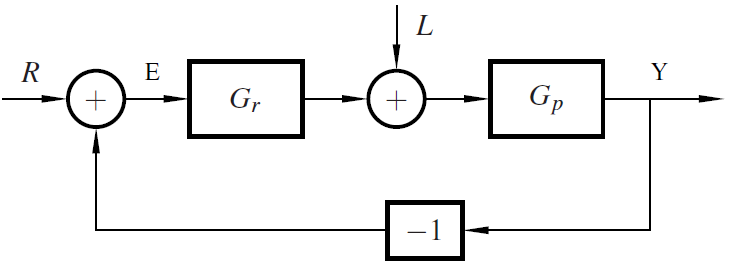
\includegraphics[width=1.0\textwidth]{res/eldiagram.png}

\end{center}
\vfill

\newpage
\vfill
\subsection{Bella Scala}
\textit{Mel: Bella Notte}\\
\index[alfa]{Bella Scala}
\index[anfa]{Åh detta språk, detta ljuvliga språk...}
\begin{parse lines}[\noindent]{#1\\}

Åh detta språk, detta ljuvliga språk,
som vi kallar bella Scala!

Se vilken syn alla uttryck i skyn,
detta ljuva bella Scala!

Fjärran från det du älskar blir koden ödsligt tom,
men i dess närhet sluts du in i dess trolska rikedom.

Åh, åh detta språk, det är ungdomens språk,
som vi kallar bella Scala!
\end{parse lines}
\vfill
\noindent\textit{Framfördes för första gången av tillträdande Inspektor och Inspektrix under Skiphtesgasquen 2023.}\\
\newpage
